\documentclass[a4paper, 12pt]{article}
\usepackage[utf8]{inputenc}
\usepackage{hyperref}
\usepackage{tabularx}
\usepackage{todonotes}
\usepackage{floatpag}
\usepackage[a4paper,bindingoffset=0.2in,
            left=0.8in,right=0.8in,top=1.4in,bottom=1.4in,%
            footskip=.48in]{geometry}



\title{Relazione progetto Machine Learning \\
    \large Appello Febbraio 2021}

\author{Gabriele Maria Bucosse 869940 \\ Ruggero Panzeri 874975\\ Davide Rendina 830730}
\date{19, February 2021}

\begin{document}

\newcommand{\imagespace}{\vspace{0.4cm}}

\maketitle

\newpage

\tableofcontents

\newpage

\section{Introduzione}
% Obiettivo elaborato
    L'obiettivo di questo elaborato è la presentazione del progetto svolto di \textit{machine learning}, relativo alla classificazione di differenti varietà di vino. Nella relazione sono incluse le fasi di esplorazione, generazione dei modelli, esperimenti e calcolo delle performance. \\
% Descrizione del dataset e del dominio
    Il dataset scelto per lo svolgimento del progetto è \textit{Red Wine Quality} [Cortez et al., 2009], disponibile sulla piattaforma \textit{\href{https://archive.ics.uci.edu/ml/datasets/wine+quality}{UCI Machine Learning Repository}}. Il dataset è relativo alle varianti del vino portoghese \textit{Vinho Verde} e include 11 covariate di input, che presentano valori basati su alcune rilevazioni fisico-chimiche, e 1 di output, il cui valore è ottenuto stabilito combinando i dati di sensoristica e almeno 3 valutazioni fatte da esperti vinicoli. Le singole \textit{feature} sono approfondite nella successiva tabella (\ref{tab:features}).
    
    Per lo svolgimento del progetto, sono state svolte diverse attività. La prima fase ha riguardato l' esplorazione del \textit{dataset} attraverso alcuni grafici, analisi di covariate e informazioni ottenute dalla \textit{PCA}. Successivamente, sono stati addestrati e testati 6 differenti modelli per effettuare la classificazione dei vini. In base ai risultati ottenuti sono state calcolate diverse metriche e, analizzando i valori ottenuti, è stato infine possibile effettuare un confronto riguardante le performance dei vari modelli.
    
% Descrizione delle singole feature
        \begin{table}[h!]
        \begin{tabularx}{\textwidth}{|l|X|}
            \hline
             \textbf{Feature} & \textbf{Descrizione} \\ \hline
             Fixed acidity & La maggior parte degli acidi del vino, fissi o non volatili (che non evaporano facilmente) \\ \hline
             Volatile acidity & La quantità di acido acetico nel vino, che a livelli troppo alti può portare a un sapore sgradevole di aceto \\ \hline
             Citric acid & Presente in piccole quantità, l'acido citrico può aggiungere "freschezza" e sapore ai vini \\ \hline
             Residual sugar & La quantità di zucchero rimanente dopo lo stop della fermentazione, è raro trovare vini con meno di 1 grammo/litro e i vini con più di 45 grammi/litro sono considerati dolci \\ \hline 
             Chlorides & La quantità di sale nel vino\\ \hline
             Free sulfur dioxide & La forma libera di SO2 esiste in equilibrio tra SO2 molecolare (come gas disciolto) e ione bisolfito; previene la crescita microbica e l'ossidazione del vino \\ \hline
             Total sulfur dioxide & Quantità di forme libere e vincolate di S02; a basse concentrazioni, SO2 è per lo più non rilevabile nel vino, ma a concentrazioni superiori a 50 ppm, SO2 diventa evidente all'odore e al gusto del vino\\ \hline
             Density & La densità dell'acqua è influenzata dalla percentuale di alcol e dalla quantità di zucchero\\ \hline
             pH & Descrive quanto è acido o basico un vino su una scala da 0 (molto acido) a 14 (molto basico); la maggior parte dei vini è compresa tra 3-4 sulla scala del pH \\ \hline
             Sulphates & Additivo per vino che può contribuire ai livelli di anidride solforosa (S02), che agisce come un antimicrobico e antiossidante \\ \hline
             Alcohol & Percentuale di alcool contenuta nel vino\\ \hline
             \textbf{Quality} & Rappresenta la \textbf{variabile target} del dataset e indica la qualità del vino, basata sui dati delle feature presentate in precedenza. Il punteggio è rappresentato da un valore nel range 1-10. \\ 
             \hline
        \end{tabularx}
        \caption{Descrizione delle feature presenti nel dataset}
        \label{tab:features}
        \end{table}
        
        \clearpage

\section{Analisi del dataset}
In questo capitolo viene approfondita la fase di analisi del dataset, organizzata in 2 differenti sezioni che descrivono rispettivamente le attività svolte di esplorazione iniziale e \textit{PCA}. 

Obiettivo della fase iniziale di esplorazione è il controllo riguardante la correttezza del \textit{dataset} caricato e l'analisi delle covariate e le relazioni che intercorrono tra esse. La \textit{PCA} invece, è stata svolta per effettuare un ulteriore studio sulle relazioni tra le covariate ma soprattutto al fine di ridurre la dimensionalità dei dati e contestualmente il loro rumore.

\subsection{Esplorazione del dataset} 
    Inizialmente sono state visualizzate le prime righe del \textit{dataset} (figura \ref{fig:out_head}), per effettuare una prima esplorazione delle variabili e valori presenti. Come è possibile osservare dal grafico, i vini sono descritti solamente da \textit{feature} numeriche. Si può notare inoltre che il \textit{dataframe} presenta esattamente 12 covariate, numero che coincide con quanto indicato nella descrizione del \textit{dataset} \footnote{\href{https://archive.ics.uci.edu/ml/datasets/wine+quality}{UCI Machine Learning: Wine Quality}}. 
    Un ulteriore controllo sulla dimensionalità dei dati ha fornito risultati relativi a numero di colonne (12) e istanze caricate (1599) che hanno trovato anch'essi corrispondenza con quanto dichiarato nella descrizione del dataset. 
    
    \imagespace
    \begin{figure}[h]
        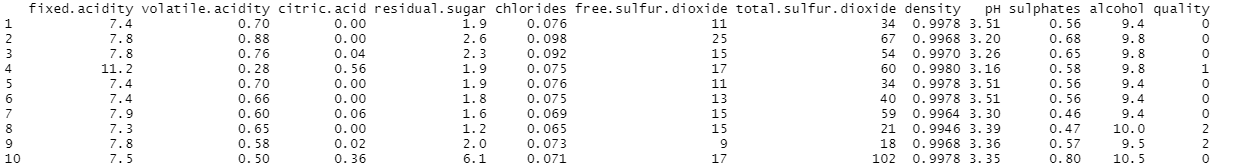
\includegraphics[width=0.95\textwidth]{img/head(wine.data)}
        \centering
        \caption{Prime righe del dataframe}
        \label{fig:out_head}
    \end{figure}
    \imagespace
    
    Successivamente è stata controllata anche la presenza di valori \textit{NA}, che ha dato esito negativo (0 \textit{NA} riscontrati) come già indicato nella descrizione del \textit{dataset}. Questo risultato indica che non è necessaria nessuna politica per la gestione di valori mancanti.
    Infine è stato effettuato un controllo per analizzare la struttura del \textit{dataset} e le tipologie di dati presenti, che ha evidenziato come tutte le covariate fossero di tipo numerico (sia discrete che continue) (figura \ref{fig:out_sapply}). 
    
    I risultati ottenuti da questa esplorazione preliminare ci permettono quindi di affermate che durante il caricamento del dataset non è presente alcun errore, in quanto tutti i valori ottenuti hanno avuto riscontro positivo con quanto dichiarato nella panoramica del dataset.
    
    \begin{figure}[h]
        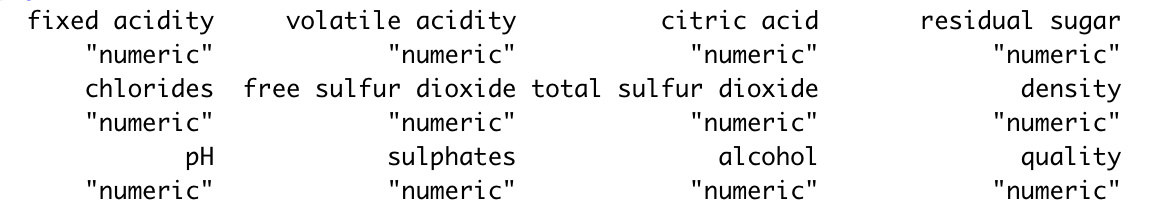
\includegraphics[width=0.9\textwidth]{img/Output_sapply().png}
        \centering
        \caption{Tipi di valori presenti nelle covariate}
        \label{fig:out_sapply}
    \end{figure}
    
    %variabile target e bilanciamento
    Al termine dei controlli riguardanti la correttezza dei dati caricati è stata scelta la covariata \textit{quality} come variabile target, poiché considerata come la più significativa per la predizione (oltre ad essere indicata come tale nella descrizione del dataset). Successivamente è stata controllata attraverso un \textit{barplot} la sua distribuzione dei valori (figura \ref{fig:out_barplot}), dal quale emerge che le istanze siano fortemente sbilanciate. Infatti, la maggior parte dei vini che ha qualità tra i valori 5-6 (82\% delle istanze) e una minoranza che invece presenta qualità bassa (4\%) oppure alta (14\%). 
    Nel dataset inoltre non è presente alcuna istanza con valori 1-2 oppure 9-10. La distribuzione della variabile riflette la distribuzione dei vini nel mondo reale, che vede quelli di qualità media in numero significativamente maggiore rispetto a quello di cattiva e buona qualità. 
    
    \imagespace
    \begin{figure}[!h]
        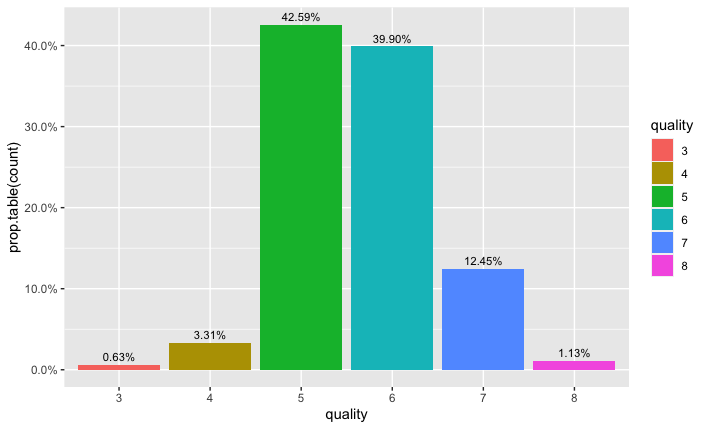
\includegraphics[width=0.9\textwidth]{img/Barplot_quality.png}
        \centering
        \caption{Distribuzione dei valori della feature quality}
        \label{fig:out_barplot}
    \end{figure}

    Dopo aver riscontrato questa distribuzione delle classi abbiamo scelto di ridurre il loro numero, al fine di facilitare i modelli di riconoscimento nella loro classificazione. Per effettuare questa suddivisione, sono state valutate diverse strategie:
    \begin{enumerate}
        \item Ridurre le classi totali da 10 a 5, accoppiando quindi le classi vicine (1-2, 3-4, 5-6, 7-8, 9-10). Il risultato sarebbero quindi state solamente 3 classi (siccome 1-2 e 9-10 non sono presenti), ma le istanze risulterebbero comunque fortemente sbilanciate (14\%, 82\% e 4\% - in ordine di qualità)
        
        \item Trasformare il problema a un problema binario, considerando le classi vini insufficienti (qualità minore di 6) e sufficienti (qualità maggiore o uguale a 6), ottenendo così due classi bilanciate (47\% e 53\% rispettivamente).
        
        \item Focalizzandoci solamente sui valori a disposizione, è possibile identificare 3 diverse classi possibili: 3-5 (qualità bassa oppure \textit{LOW}), 6 (qualità media oppure \textit{MEDIUM}) e 7-8 (qualità alta oppure \textit{HIGH}). Le classi risultano comunque sbilanciate (rispettivamente 46.5\%, 39.9\% e 13.6\%), ma la situazione è migliore rispetto a quanto analizzato nel punto 1. 
    \end{enumerate}
    Si può notare quindi come la soluzione ottimale sia quella presentata nel punto 2, con un problema binario e un bilanciamento quasi perfetto tra le classi. La nostra scelta però è ricaduta sulla terza opzione, poiché:
    \begin{itemize}
        \item Consideravamo la suddivisione binaria un po' meno significativa, dato che la divisione da noi scelta mantiene concettualmente un livello di qualità in più per la catalogazione dei vini.
        \item Ci piaceva l'idea di confrontarci con un problema multiclasse e non solo binario. 
    \end{itemize}
    
    Dopo aver scelto la suddivisione, è stata impostata a categorica la covariata \textit{quality}. La nuova distribuzione di questa feature è illustrata nel \textit{barplot} in figura \ref{fig:out_barplot3}, che fornisce anche informazioni sulla buona riuscita dell'operazione svolta. \'E possibile infatti verificare che i livelli di \textit{quality} sono 3 e non più 6 e che le percentuali cumulate corrispondono. Un ulteriore controllo sulle righe del \textit{dataframe} ha constatato che è stato modificato il numero delle istanze.
    
    \begin{figure}[!h]
        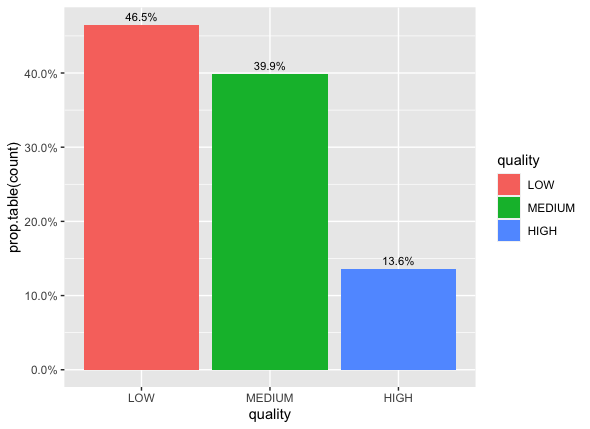
\includegraphics[scale=0.50]{img/Barplot_quality3.png}
        \centering
        \caption{Nuova distribuzione dei valori della feature quality}
        \label{fig:out_barplot3}
    \end{figure}    
    
    Sono stati visualizzati successivamente diversi grafici per l'analisi delle covariate del \textit{dataset}, al fine di comprendere la difficoltà del problema e le studiare relazioni tra le varie \textit{feature}.
    
    Per ogni covariata è stato generato un \textit{boxplot} che mette in relazione i suoi valori con quelli della variabile target. Da questi grafici evince come in realtà nessuna tra le \textit{feature} del \textit{dataset} sia in grado di effettuare una distinzione efficace tra le classi, poiché per tutte le istanze si verifica la sovrapposizione non solo dei "baffi" del grafico, ma anche dei relativi box (dove si concentra la maggior parte dei valori). Inoltre per alcune covariate sono presenti molti \textit{outliers}, che potrebbero causare problemi nella fase successiva di classificazione. 
    Dai grafici si può notare come le covariate \textit{residual.sugar} e \textit{chlorides} siano in assoluto le peggiori, in quanto hanno quasi completamente i box sovrapposti e numerosi \textit{outliers}. Un'altra covariata che presenta un numero notevole di \textit{outliers} è \textit{sulphates}. Le \textit{feature} migliori per la discriminazione (anche se comunque non presentano risultati buoni) sembrano essere \textit{alcohol} e \textit{volatile.acidity}, in quanto le uniche per le quali i box non sono molto sovrapposti, le mediane sono abbastanza lontane per tutte e tre le classi e non presentano molti \textit{outliers}.
    
    \vspace{1.4cm}
    \begin{figure}[h]
        \noindent\makebox[\textwidth]{%
        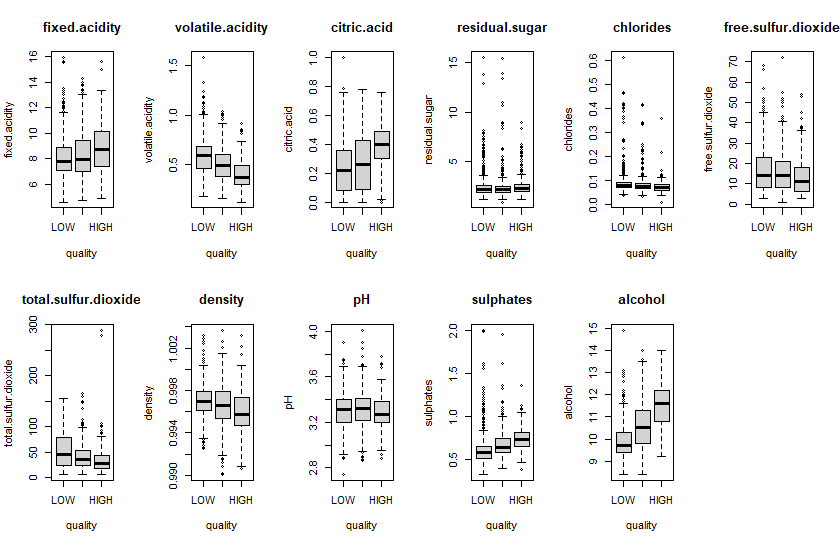
\includegraphics[scale=0.6]{img/boxplot_quality.png}}
        \centering
        \caption{Output boxplot per label}
        \label{fig:out_boxplot_label_2}
    \end{figure}
    
    \newpage
    
    %APPUNTI
    %Dobbiamo mettere in luce nella relazione: presenza di outliers che potrebbero causare qualche problema in fase di classificazione
    %Seconda info: mettendo in relazione i boxplot, vedo se gli intervalli si sovrappongono o meno -> difficoltà a distinguere, quindi quale classe si distingue meglio guardando la covariata xxx ?
    %Maggiorparte dei dati ce l'abbiamo dove c'è il box, però attenzione alle code che si sovrappongono: se si sovrappongono, non è netta la suddivisione
    %Pallini: ouliers - a seconda dell'intervallo di confidena hanno prob bassa di occorrere all'interno della variabile
    
    Anche attraverso la visualizzazione dello \textit{scatterplot} per tutte le covariate (figura \ref{fig:out_scatterplot_matrix}), ci si può rendere conto come in realtà nessuna coppia di esse sia in grado di effettuare una divisione efficace delle classi. Le classi infatti risultano per tutte le combinazioni di molto sovrapposte, e questa condizione è indice del fatto che potrà essere complicato avere una suddivisione efficace delle classi. Le covariate che sembrano suddividere meglio in questo caso le tre classi sembrano essere \textit{free.sulfur.dioxide} e \textit{total.sulfur.dioxide}. Anche osservando la distribuzione delle varie \textit{feature} (figura \ref{fig:out_featureplot}) si può osservare come i valori risultino fortemente sovrapposti e per alcune covariate sono perfettamente sovrapposte anche le distribuzioni stesse.
    
    \vspace{1.2cm}
    \begin{figure}[!h]
        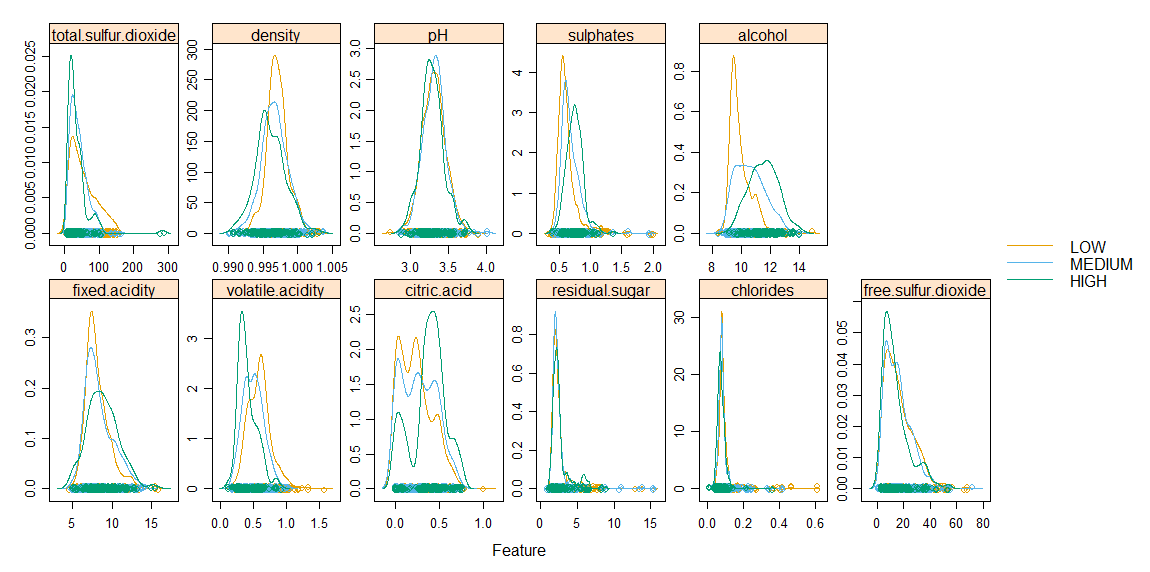
\includegraphics[width=\textwidth]{img/Rplot.png}
        \centering
        \caption{Distribuzione delle variabili}
        \label{fig:out_featureplot}
     \end{figure}   
         
    \newpage
    \begin{figure}[!h]
        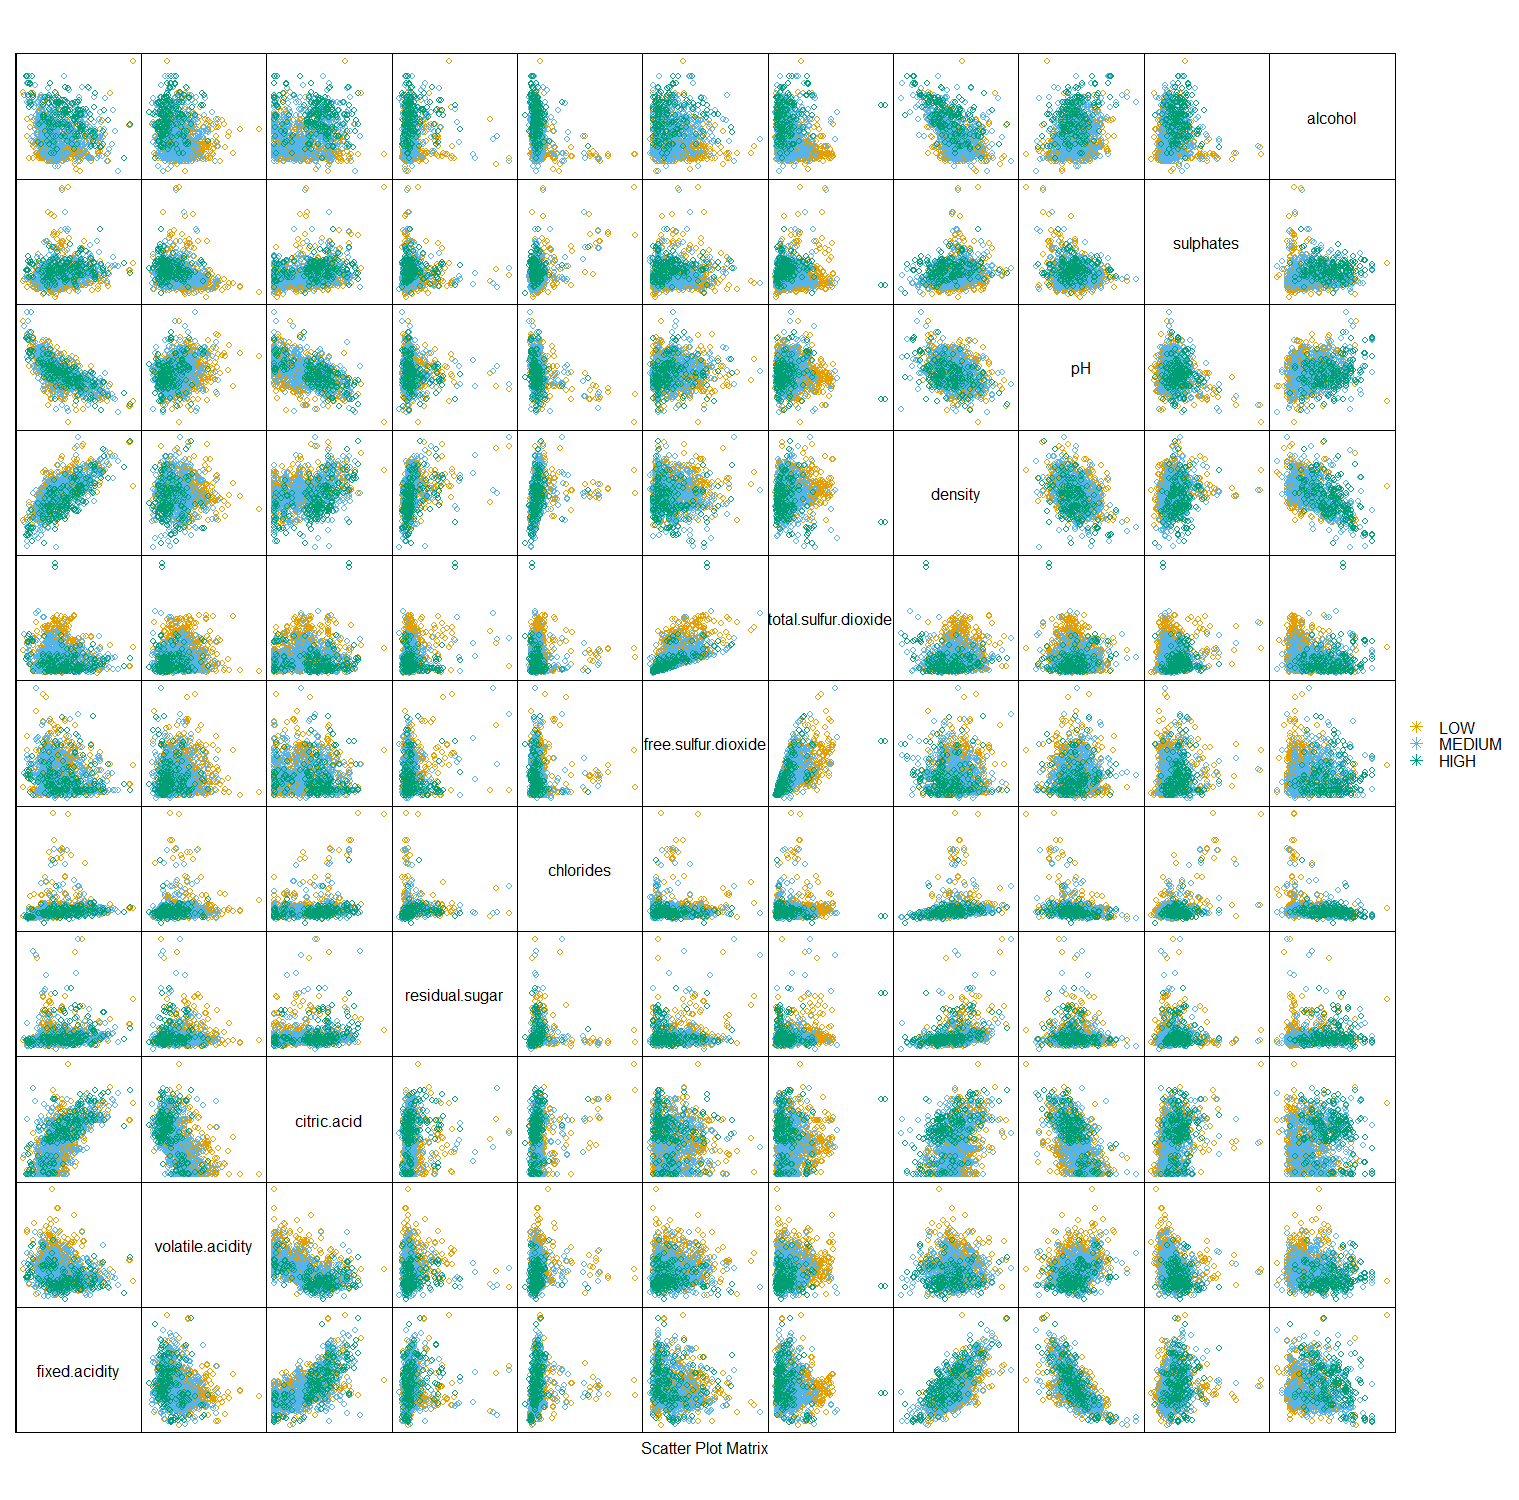
\includegraphics[width=0.9\textwidth]{img/scatterplot_2000.png}
        \centering
        \caption{Scatterplot Matrix}
        \label{fig:out_scatterplot_matrix}
    \end{figure}
    
    \vspace{1cm}
    %TEORIA pallino è l'istanza, serve per capire a coppie di covariate quali siano quelle che dividono meglio una precisa classe
    % Serve per capire quali covariate permettono di discriminare meglio le classi
    
    %\paragraph{Boxplot univariato} a me sembra inutile, risento lab 2 da 58:00 circa
    
    %\paragraph{featurePlot} capire bene (cercando su internet) cosa ci dice. Serve a vedere come si ditribuiscono le covariate
    
%Descrizione del training set: analisi esplorativa del training set (analisi delle covariate e/o PCA)
    % Diagrammi utilizzati per l'esplorazione
    
\subsection{PCA: Principal Component Analysis}
% Note that, the PCA method is particularly useful when the variables within the data set are highly correlated. Correlation indicates that there is redundancy in the data. Due to this redundancy, PCA can be used to reduce the original variables into a smaller number of new variables ( = principal components) explaining most of the variance in the original variables. 
    Al fine di studiare in maniera più approfondita la correlazione tra le variabili e contestualmente provare a ridurre la dimensionalità del dataset e il rumore nei dati, è stata effettuata anche la \textit{Principal Component Analysis}. In un \textit{dataset} non tutti gli attributi sono assolutamente informativi (si può vedere anche dai vari grafici visti finora) ed alcuni possono anche risultare dannosi, aumentando solamente la complessità del modello e rischiando in alcuni casi di confonderlo. Per questi motivi, è stato deciso di utilizzare questo metodo. 
    
    Dopo aver effettuato la \textit{PCA}, è stata osservata la varianza rappresentata da ogni componente. Come si può vedere dagli autovalori presenti nella figura \ref{fig:out_eig}, non sono presenti componenti che singolarmente spiegano una grande quantità di varianza, ma piuttosto la varianza è distribuita in maniera abbastanza omogenea tra diverse le componenti (escluse ovviamente le ultime). 
    
    \begin{figure}[!h]
        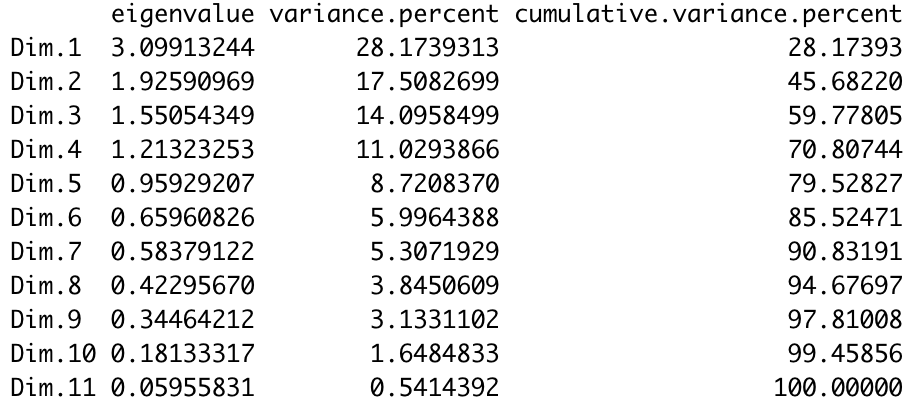
\includegraphics[width=0.7\textwidth]{img/autovalori_pca.png}
        \centering
        \caption{Autovalori PCA}
        \label{fig:out_eig}
    \end{figure} 
    
    Per scegliere quali componenti da mantenere abbiamo deciso di non considerare solamente quelle con autovalori con valore maggiore di 1 ma di scegliere in base alla varianza cumulata, al fine di mantenere un valore di varianza alto. In particolare, è stato deciso di tenere solamente 7 componenti in maniera tale da avere il 90\% della varianza totale. Per effettuare poi le operazioni successive di \textit{train} e \textit{test} è stato considerato il \textit{dataset} prodotto dalla \textit{PCA} nel nuovo spazio di indirizzamento, passando da 11 a 7 dimensioni.
    
    Analizzando le prime due dimensioni della PCA, è possibile effettuare qualche considerazione attraverso alcuni grafici. Osservando il grafico delle variabili (figura \ref{fig:out_pcavar}), si può notare come \textit{sulphates, chlorides e anche residual.sugar} siano le \textit{feature} peggio rappresentate nel nuovo spazio di indirizzamento. Riprendendo le considerazione fatte in precedenza analizzando i boxplot, si può notare come queste siano le variabili che avevamo indicato come le peggiori, sia per sovrapposizione dei valori sia per la presenza di numerosi \textit{outliers}. 
    
    \begin{figure}[!h]
        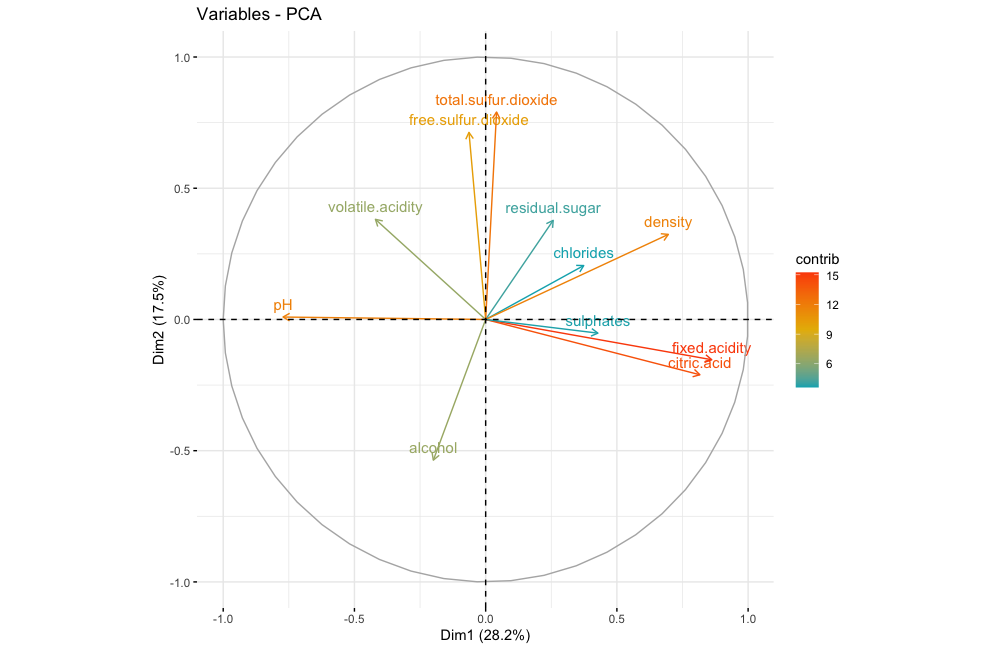
\includegraphics[width=0.9\textwidth]{img/Output_pcavar().png}
        \centering
        \caption{Output fvizpcavar()}
        \label{fig:out_pcavar}
    \end{figure}
    
    Analizzando questo grafico, si possono effettuare anche considerazioni sulla correlazione tra le variabili. Le covariate \textit{fixed.acidity, citric.acid e sulphates} risultano fortemente dipendenti tra loro, come accade per \textit{total.sulfur.dioxide e free.sulfur.dioxide} e anche \textit{chlorides e density}. In generale, la maggior parte delle variabili risulta linearmente dipendente (più o meno fortemente), in quanto le frecce sono tutte concentrate nel quadrante in alto a dx (o nelle sue vicinanze). Le \textit{feature} \textit{alcohol}, \textit{pH} e \textit{volatile.acidity} risultano invece poco correlate rispetto a tutte le altre (soprattutto \textit{alcohol}).

    Un altro grafico sul quale si possono effettuare alcune considerazioni è quello degli \textit{individuals} (figura \ref{fig:out_pcaind}).
    Si può verificare come nel nuovo spazio di rappresentazione (considerando solo le prime due dimensioni), molte istanze non vengano ben rappresentate (colorate di azzurro e verde, concentrate al centro del grafico). Inoltre dal grafico riguardante la classificazione si può osservare che le sole prime due dimensioni non siano necessarie per una suddivisione efficace delle istanze, in quanto tutti gli elementi risultano fortemente sovrapposti. 
    
    Questi risultati ci suggeriscono che anche utilizzando il nuovo spazio di indirizzamento, potremmo avere comunque problemi ad individuare le diverse classi (questo era un risultato atteso, in quanto abbiamo ridotto la varianza e comunque le due dimensioni spiegano solamente il 45\% della varianza totale). Avendo rimosso però una parte di informazioni ridondanti, potremmo avere come beneficio un aumento della precisione dei modelli, nonché una minore complessità degli stessi. 
    
    \vspace{0.6cm}
    \begin{figure}[!h]
        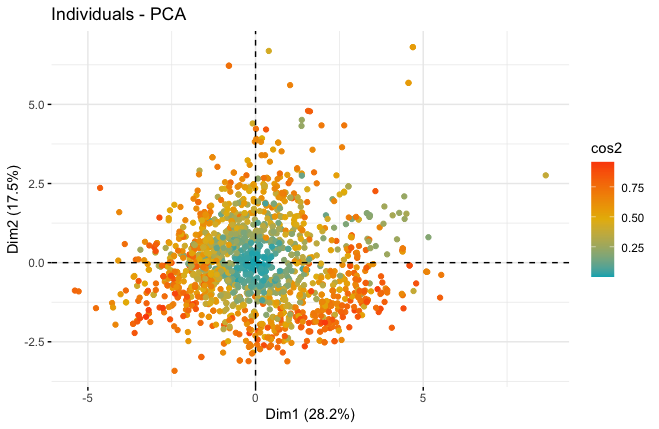
\includegraphics[width=.5\textwidth]{img/individuals_pca_1.png}%
        \qquad
        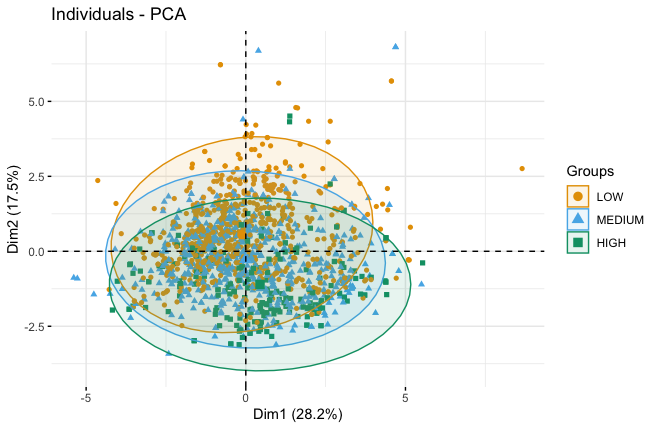
\includegraphics[width=.5\textwidth]{img/individuals_pca_2.png}
        \caption{Individuals PCA}
        \label{fig:out_pcaind}
    \end{figure}
    
    \newpage


\newpage
\section{Esperimenti}
    Questo capitolo approfondisce la parte del progetto relativa ai modelli e agli esperimenti effettuati. In particolare vengono motivate le decisioni effettuate nella scelta e addestramento dei modelli, descritto il \textit{workflow} seguito per ogni modello e analizzati i risultati ottenuti.
    
    \subsection{Scelta dei modelli}
        Per identificare i modelli più adatti, è stato scelto un approccio che prevede il confronto tra sei diversi modelli di \textit{machine learning}, per confrontare le loro prestazioni e identificare i migliori. In particolare, abbiamo utilizzato per i nostri esperimenti una rete neurale, un albero di decisione, \textit{naive bayes} e tre diversi modelli di \textit{SVM} (con \textit{kernel} rispettivamente lineare, polinomiale, radiale). Abbiamo escluso solamente l'algoritmo \textit{k-means}, in quanto il nostro desiderio era effettuare solamente approcci supervisionati, avendo anche a disposizione le \textit{label} per le istanze. È stato possibile scegliere questo tipo di approccio poiché il dataset utilizzato presenta un numero esiguo di istanze e \textit{feature}, e il rispettivo \textit{train} dei vari modelli non è molto pesante in termini di tempo e risorse utilizzate. Se invece avessimo avuto un numero notevolmente maggiore di istanze e covariate, sarebbe stato più complicato sotto certi aspetti effettuare queste operazioni per tutti quanti i modelli.
        
    \subsection{Attività svolte per ogni modello}
        Per ogni modello introdotto in precedenza, si è seguito il seguente \textit{workflow}:
        \begin{enumerate}
            \item Addestramento attraverso il \textit{trainset} 
            \item Predizione sui dati contenuti nel \textit{testset}
            \item Calcolo delle metriche per il modello
            \item Calcolo della curva ROC multiclasse
        \end{enumerate}
        
        \paragraph{Train del modello e predizione} 
        Per la suddivisione dei dati in \textit{trainset} e \textit{testset} è stato deciso di selezionare il 30\% delle istanze complessive (480 istanze) in modo da rispettare la distribuzione delle istanze in base al loro valore di \textit{quality}. 
        
        L'addestramento del modello è stato effettuato svolgendo la \textit{3-repeated 10-fold cross validation}, attraverso il parametro \textit{trainControl} della funzione \textit{caret::train}. Questa opzione ci ha permesso di fare il \textit{tuning} ottimale dei parametri dei vari modelli, in quanto effettua diverse iterazioni con valori differenti al fine di trovare la misura che permette di ottimizzare la misura specificata. Per effettuare questa ottimizzazione, è stata scelta la misura di \textit{AUC}.
        
        Le predizioni invece sono state effettuate utilizzando il modello generato dal \textit{training} e il \textit{testset} precedentemente suddiviso.
    
        \paragraph{Calcolo delle metriche} Per ogni predizione effettuata, è stata poi calcolata la matrice di confusione. Il calcolo della matrice ci ha quindi permesso di determinare le differenti metriche per ogni modello generato. In particolare è stato possibile calcolare la \textit{accuracy} su tutta la matrice di confusione e \textit{precision, recall e f-measure} per ogni classe del problema. I risultati di questa fase verranno discussi nella sezione successiva.

        \paragraph{Calcolo della curva ROC} \'E stato effettuato infine il calcolo della curva \textit{ROC} e del relativo valore di \textit{AUC}. In quanto problema multiclasse, sono state generate 5 diverse curve per ogni modello: 3 relative alle classi del problema (\textit{LOW, MEDIUM, HIGH}) e le altre 2 invece alla \textit{micro average} e \textit{macro average} dei valori ottenuti.
        
        \subsubsection{Repeated 10-fold cross validation}
        Per effettuare il \textit{train} dei modelli, sono state valutate diverse tipologie differenti di metodi di \textit{resampling}. In particolare, sono state testate le prestazioni per \textit{10-fold cross validation} (d'ora in poi \textit{10-fold CV}) e \textit{k-repeated 10-fold cross validation} (considerate 10, 5 e 3 ripetizioni).
        
        Dopo aver testato i nostri modelli utilizzando la \textit{10-fold CV}, è stato deciso di sperimentare anche la \textit{10-fold CV k-repeated}. Partendo da un valore di ripetizioni k=10, abbiamo successivamente diminuito il numero di ripetizioni a k=5 e k=3. Durante lo svolgimento di queste tre prove, non sono stati riscontrati miglioramenti significativi utilizzando diversi valori di k, soprattutto non tali da giustificare l'aumento di complessità computazionale temporale.\\
        
        \begin{table}[h]
            \begin{tabular}{| c | c | c | c | c |}
                \hline
                 \textbf{Modello} & \textbf{10-fold CV} & \textbf{3 repeated} & \textbf{5 repeated} & \textbf{10 repeated}\\ 
                 \hline
                 Albero decisionale & 1.41 & 3.09 & 4.91 & 8.67 \\
                 Naive Bayes & 1.36 & 3.05 & 4.44 & 8.08 \\
                 Svm lineare & 2.96 & 3.33 & 5.03 & 9.23 \\
                 Svm polinomiale & 27.77 & 81.91 & 138.83 & 272.82 \\
                 Svm radiale & 4.86 & 13.08 & 20.97 & 41.13 \\
                 Rete neurale & 8.23 & 24.00 & 38.24 & 74.36 \\
                 \hline
            \end{tabular} 
            \caption{Tempi di calcolo con diversi metodi di resampling}
        \end{table}
        
        %Analizzando i valori ottenuti è stato osservato che con k=3 ripetizioni, venivano introdotti miglioramenti alle metriche di \textit{accuracy}, \textit{precision}, \textit{recall} e \textit{F1} durante il riconoscimento della classe \textit{HIGH}. Per questo motivo è stata utilizzata una \textit{10-fold CV 3-repeated}, considerato anche che non si è verificato un significativo aumento della complessità computazionale temporale. 
        
        I grafici successivi (figure \ref{fig:out_confrontoavg} e \ref{fig:out_confrontohigh}) mettono a confronto i valori delle metriche ottenuti attraverso la \textit{10-fold CV} (viola) con quelli risultanti dalla \textit{10-cross CV 3-repeated} (verde), per ogni metrica e modello. Sono presentati in particolare due grafici, uno relativo alla classe \textit{high} e l'altro al valore di \textit{macro average} tra tutte e tre le classi; i grafici delle altre due classi (\textit{medium, low}) non sono stati considerati per questo confronto in quanto poco significativi.
        
        \begin{figure}[!h]
            \noindent\makebox[\textwidth]{%
            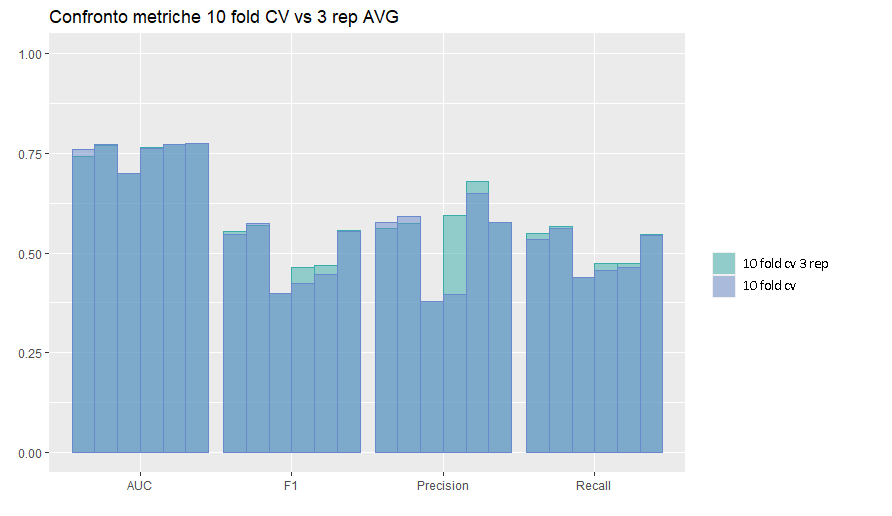
\includegraphics[width=\textwidth]{img/confronto_AVG.png}}
            \centering
            \caption{Confronto relativo alla media}
            \label{fig:out_confrontoavg}
        \end{figure}
    
        \begin{figure}[!h]
            \noindent\makebox[\textwidth]{%
            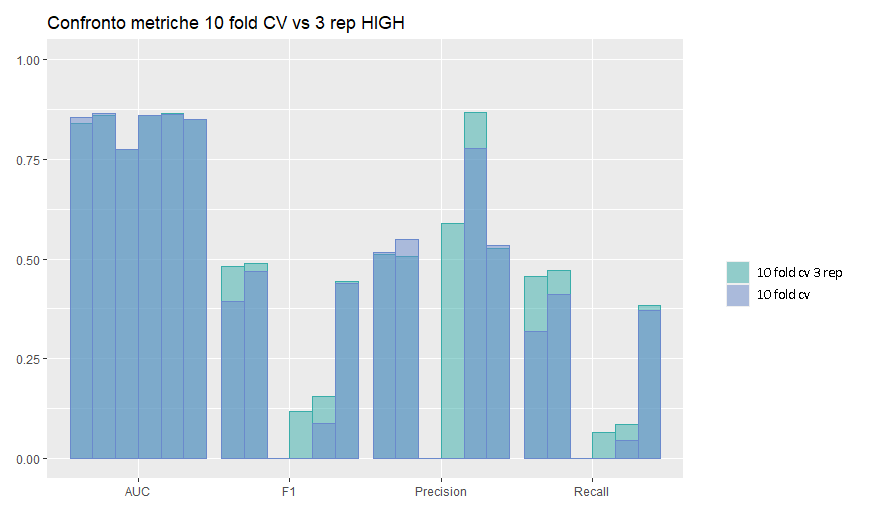
\includegraphics[width=\textwidth]{img/confronto_HIGH.png}}
            \centering
            \caption{Confronto relativo alla classe high}
            \label{fig:out_confrontohigh}
        \end{figure}
        
        \newpage
        Dai valori di \textit{macro average} (\ref{fig:out_confrontoavg}) emerge che ci sono stati piccoli cambiamenti in positivo per diversi modelli per le metriche \textit{F1}, \textit{recall} e soprattutto \textit{precision}. I cambiamenti più interessanti possono essere però osservati nel grafico successivo (\ref{fig:out_confrontohigh}), dove emerge un significativo miglioramento per tutte le metriche considerate. Uno dei modelli considerati inoltre non era in grado di classificare correttamente alcuna istanza per la classe \textit{high}, situazione che invece è cambiata con l'utilizzo della \textit{10-fold CV 3-repeated}. Questi motivi hanno quindi spinto all'adozione della \textit{10-fold CV 3-repeated} a favore della \textit{10-fold CV} senza ripetizioni.
        
        %Come miglioramento ulteriore abbiamo testato la validità di una \texit{10fold cv k repeated} invece di una \textit{10fold cv}. Siamo partiti da una \texit{10 fold cv 10 repeated} e dimezzato fino ad una \texit{10fold cv 3 repeated}, abbiamo riscontrato che in termini di miglioramento non ci sono significative differenze per il nostro modello fra 3 5 e 10 repeated, sopratutto non  così significative da giustificare l'aumento di complessità computazionale temporale. 
        %Quindi abbiamo deciso di implementare una \texit{10 fold 3 repeatet} che introduce miglioramenti in accuracy, precision, recall e F1 per la maggior parte dei modelli.
        
        \subsubsection{Downsampling}
            Essendo il numero di istanze delle varie classi sbilanciato, è stato osservato che il comportamento dei modelli risultava migliore sulla classe di maggioranza (\textit{LOW}) rispetto alle altre classi con meno istanze (\textit{MEDIUM, HIGH}). Per cercare di migliorare le prestazioni per le classi meno numerose, è stato effettuato l'addestramento delle stesse applicando una strategia di \textit{downsampling}. \'E stato scelto di utilizzare questa tecnica a favore di altre per due motivi principali: 
            \begin{itemize}
                \item Le altre tecniche creavano un numero molto alto di istanze per le classi di minoranza e andavano ad inserire numerosi istanze che non riflettevano la realtà.
                \item Essendo i valori di tutte le \textit{feature} molto vicini tra le varie classi, la creazione di altre istanze avrebbe rischiato di confondere ulteriormente il modello.
            \end{itemize}
            Analizzando i risultati ottenuti , abbiamo verificato che questa strategia ci ha permesso di migliorare le prestazioni in termini di riconoscimento della classe di minoranza \textit{HIGH}, ma ha anche peggiorato notevolmente le prestazioni per la classe \textit{MEDIUM} e anche i valori di \textit{macro average} sono risultati leggermente inferiori. Per questi motivi, è stato deciso quindi di non adottare nessuna strategia di questo tipo.

    \subsection{Analisi dei risultati ottenuti}
    La prima metrica che è stata considerata per effettuare l'analisi è la \textit{accuracy}, i quali valori sono riportati nel grafico \ref{fig:out_accuracyplot} insieme all'intervallo di confidenza. Come si può osservare dalla figura, tutti i modelli riportano sia valori che intervalli quasi sovrapposti. Considerando però che stiamo analizzando un problema multiclasse questi valori da soli non sono sufficienti per valutare la bontà del modello, in quanto non tengono conto delle diverse classi presenti. Per effettuare quindi analisi più accurate, dobbiamo considerare anche ulteriori metriche.
    
    \begin{figure}[h]
        \noindent\makebox[\textwidth]{%
        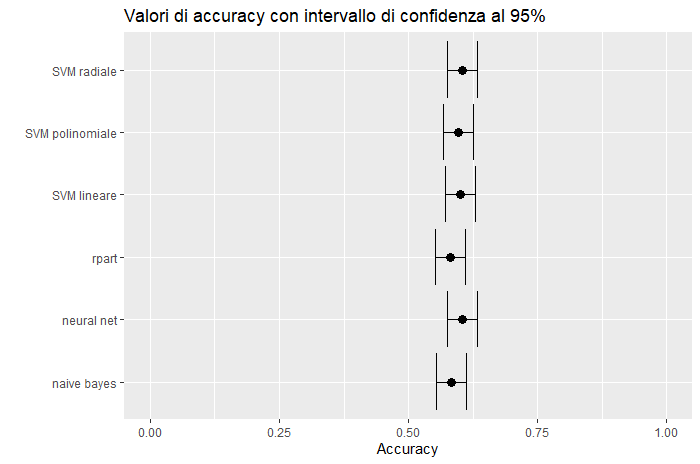
\includegraphics[scale=0.70]{img/plot_accuracy.png}}
        \centering
        \caption{Accuracy dei diversi modelli}
        \label{fig:out_accuracyplot}
    \end{figure}
    
    Avendo scelto un problema multiclasse, abbiamo ottenuto diversi valori per le metriche calcolate. Per la visualizzazione dei valori di \textit{AUC} e metriche, sono stati utilizzati grafici a barre. Sono stati generati in tutto 4 grafici di questa tipologia, 3 relativi alle classi del problema mentre il quarto prende in considerazione la \textit{macro average}, ed oguno di essi mette in relazione per ogni misura i risultati ottenuti dai vari classificatori (figura \ref{fig:out_metrics}). 
    Abbiamo valutato questa visualizzazione come la migliore poiché ci ha permesso di avere un numero minore di grafici rispetto ad altri approcci e contestualmente poter confrontare semplicemente le prestazioni per singola classe, che è stata reputata come l'informazione migliore per effettuare la valutazione.
    
    Per aggregare le metriche abbiamo optato per l'utilizzo della \textit{macro average} a dispetto della \textit{micro average}, poiché non desideravamo dare più importanza a nessuna classe nonostante lo sbilanciamento delle istanze. Avendo valutato poi singolarmente le prestazione per ogni classe e non solo il valore aggregato, è stato comunque tenuto conto del loro sbilanciamento.
    
    Osservando le metriche di \textit{marco average} si può osservare come le prestazioni medie per tutti i classificatori siano molto simili. I modelli che presentano valori aggregati peggiori sono gli alberi di decisione e, in maniera minore, \textit{SVM} lineare. 
    Al fine di analizzare nel dettaglio le cause che portano a questa differenza con gli altri modelli, è necessario guardare i valori ottenuti per ogni singola classe. In generale, si può affermare che si siano ottenute prestazioni buone sulla classe \textit{LOW} (le metriche oscillano tra il 70\% e 75\%), mentre per le altre due classi i valori sono molto meno buoni, con le metriche che oscillano intorno al 50\% per entrambe le classi. Si può osservare inoltre come per la classe di minoranza (\textit{HIGH}) alcuni classificatori non siano stati in grado di rilevare alcuna istanza. In particolare, per quanto riguarda l'albero di decisione sono stati ottenuti valori nulli.
    Questa variazione di valori può essere causata dallo sbilanciamento delle istanze in relazione alle tre classi. Come presentato in precedenza però, anche tecniche come \textit{downsampling} non sono riuscite migliorato la situazione. Si può quindi pensare che queste difficoltà siano anche dovute al fatto che i dati non siano facilmente separabili.
    
    \newpage
    
    \begin{figure}[!h]
        \noindent\makebox[\textwidth]{%
        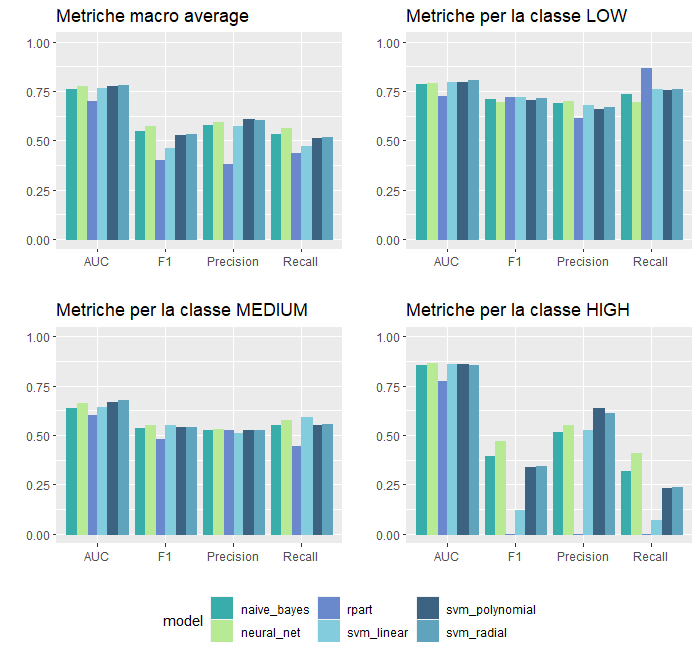
\includegraphics[scale=0.78]{img/final_metrics/finalmetrics.png}}
        \centering
        \label{fig:out_metrics}
        \caption{Metriche calcolate raggruppate per classe}
    \end{figure}

    Per ogni modello è stato anche generato il grafico relativo alle curve ROC, che rappresenta le 3 curve per le rispettive classi del problema e ulteriori 2 curve relative alle curve calcolate attraverso i valori aggregati di \textit{micro e macro average}.
    Analizzando i grafici e i valori di \textit{Area Under Curve} presentati nei grafici precedenti (\ref{fig:out_metrics}), si può osservare come le curve siano in generale molto simili tra loro e non ci sia grande discrepanza tra i differenti valori di \textit{AUC}. La curva di \textit{rpart} però risulta leggermente peggiore rispetto alle altre, e si può inoltre osservare che gli alberi presentino i valori di \textit{AUC} più bassi tra tutti i modelli.
    
    Per ogni modello inoltre emerge una differenza fra la curva relativa alla classe \textit{MEDIUM} e le altre 4. Questo valore indica la difficoltà dei modelli durante la classificazione di questo tipo di istanze, e anche in precedenza analizzando le metriche calcolate era già stato sottolineato questo aspetto. La classe \title{MEDIUM} ha performance peggiori rispetto alla classe \title{HIGH} poiché in percentuale tende a sbagliare di più in riferimento al numero di istanze totali.
    
    \newgeometry{left=0cm,right=1cm, top = 0.8cm}
    \thisfloatpagestyle{empty}
    
    \begin{table}[]
    \begin{tabular}{cc}
    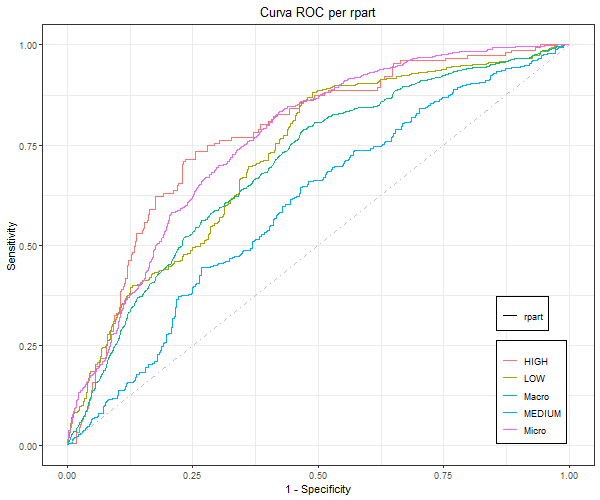
\includegraphics[width=.5\textwidth]{img/roc/roc_rpart.png} &
    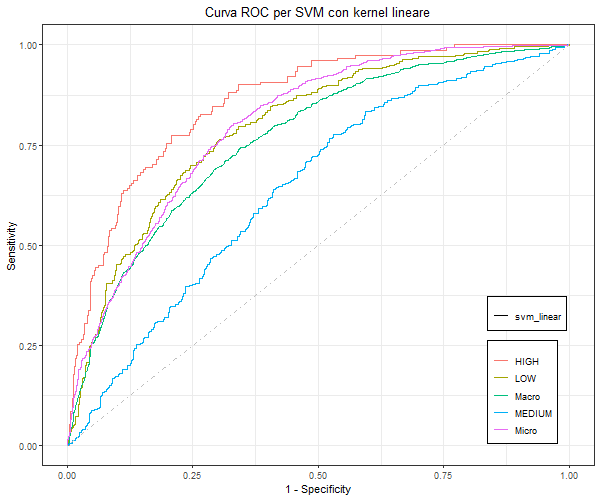
\includegraphics[width=.5\textwidth]{img/roc/roc_svml.png} \\
    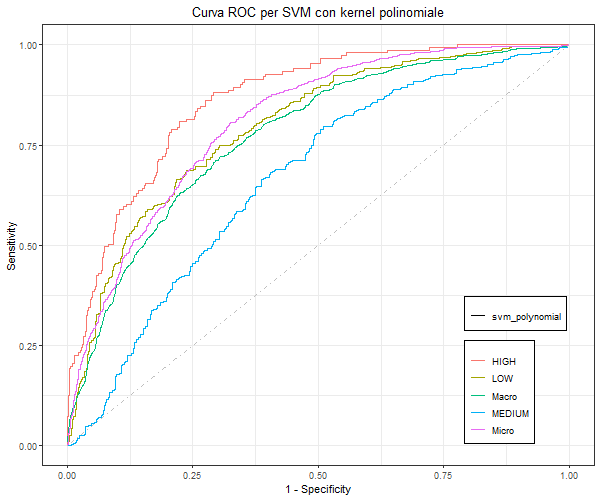
\includegraphics[width=.5\textwidth]{img/roc/roc_svmp.png} &
    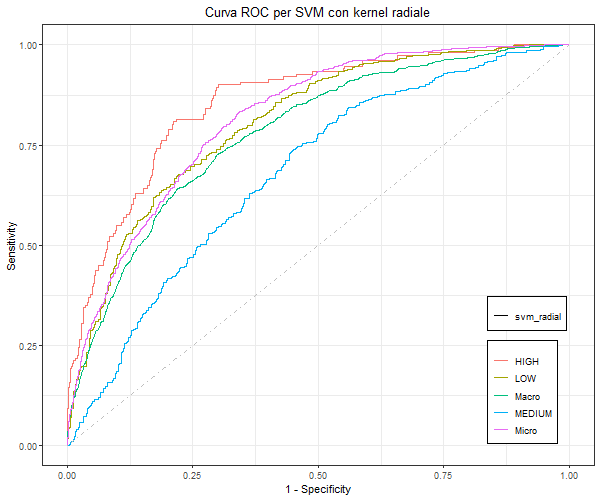
\includegraphics[width=.5\textwidth]{img/roc/roc_smvr.png} \\
    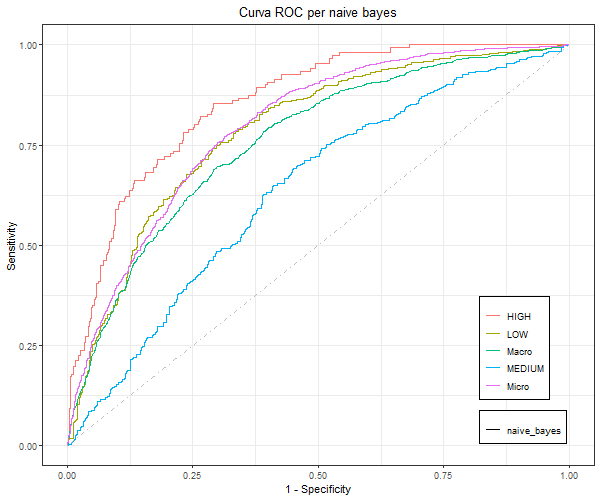
\includegraphics[width=.5\textwidth]{img/roc/roc_nb.png} &
    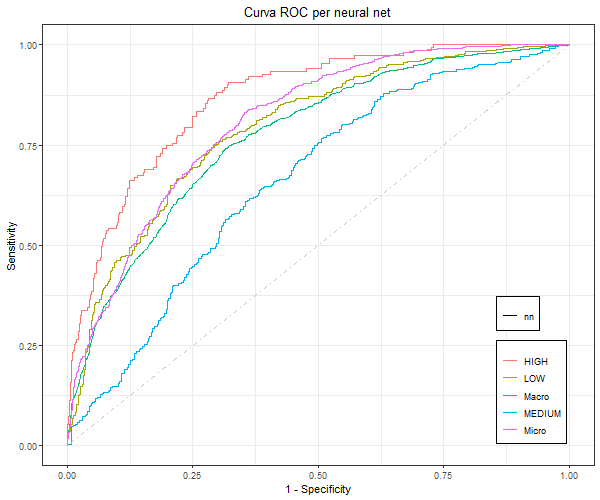
\includegraphics[width=.5\textwidth]{img/roc/roc_nn.png} \\
    \end{tabular}
    \caption{Curve ROC per tutti i modelli e per tutte le classi}
    \end{table}
    
    \restoregeometry
    \newpage
    
    Un ulteriore analisi delle prestazioni dei modelli si può effettuare considerando i loro tempi di \textit{training} e \textit{prediction}, illustrati nella tabella successiva (\ref{tab:timing}).
    Come si può osservare dai dati riportati albero decisionale, \textit{naive bayes} e SVM lineare sono i modelli più rapidi (circa 3sec), mentre il più lento in assoluto è SVM polinomiale (27x volte più lento di questi tre). SVM radiale e rete neurale invece presentano tempi più alti rispetto ai più veloci rispettivamente di 4x volte e 8x volte.
    
    Si può notare come ovviamente i modelli più semplici abbiano prestazioni ottime mentre quelli più complessi abbiamo bisogno di maggiore tempo per l'addestramento e la predizione. Si deve comunque considerare che per quanto ci sia una grande discrepanza tra i modelli, avendo utilizzato un dataset con un numero ridotto di istanze e covariate i tempi sono comunque bassi (massimo un minuto e mezzo).
    
    \begin{table}[h]
        \centering
        \begin{tabular}{| c | c |}
            \hline
             \textbf{Modello} & \textbf{Timing} \\
             \hline
             Albero decisionale & 3.09 \\
             Naive Bayes & 3.05 \\
             Svm lineare & 3.33 \\
             Svm polinomiale & 81.91 \\
             Svm radiale & 13.08 \\
             Rete neurale & 24.00 \\
             \hline
        \end{tabular} 
        \caption{Tempi di calcolo con diversi metodi di resampling}
        \label{tab:timing}
    \end{table}
    
    Considerando tutti gli aspetti presentati è quindi possibile quindi delineare quale siano i modelli che possano essere considerati come i migliori. Oltre alle prestazioni raggiunte, è importante considerare anche il costo per ottenerle, al fine di avere il giusto \textit{trade off} tra tempi e correttezza delle predizioni del modello.
    
    L'albero decisionale è in assoluto il modello più semplice e veloce tra quelli presentati, ma questo si traduce anche in prestazioni non ottimali. Come già presentato in precedenza infatti, non è stato in grado di classificare alcuna istanza di tipo \textit{HIGH}, oltre a non avere prestazioni come gli altri relative a tutte le altre classi. Per questo motivo, si può affermare che, nonostante i suoi pregi, non possa essere considerato in questo caso un buon classificatore.
    
    \textit{Naive Bayes} è il modello giudicato come migliore tra quelli presentati, poiché si rilevano ottime prestazioni mantenendo però bassa complessità computazionale. Come si può osservare dai grafici infatti, le sue prestazioni sono in linea con quelle degli altri classificatori più complessi ma presenta il tempo in assoluto più basso per addestramento e predizione.
    
    Un modello che ha ottenuto prestazioni inferiori rispetto agli altri è \textit{SVM} lineare, che come gli alberi ha presentato problemi di classificazione per la classe \textit{HIGH}, ma nonostante ciò è un buon \textit{trade-off} tra risultati ottenuti e complessità computazionale. Per questo può essere considerato come un discreto classificatore, nonostanze prestazioni inferiori agli altri modelli.
    
    Per quanto riguarda \textit{SVM} polinomiale invece, presenta ottime prestazioni dal punto di vista delle metriche. Il fattore che penalizza però molto questo classificatore è il tempo di addestramento e predizione, che è in assoluto quello più alto riscontrato tra tutti i modelli analizzati. Possiamo quindi considerare altri classificatori (come ad esempio \textit{naive bayes}, reti neurali e \textit{SVM} radiale) come migliori poiché, a fronte di prestazioni simili, si ha una complessità computazionale decisamente minore.
    
    \textit{SVM} radiale e reti neurali possono infine essere considerati entrambi come buoni classificatori. Per quanto riguarda il primo abbiamo ottenuto prestazioni in linea con i modelli migliori, a fronte di una complessità abbastanza bassa. La rete neurale invece, nonostante tempi di addestramento e predizione tra i più alti, è stato il modello che è stato più in grado di effettuare una discriminazione corretta delle istanze \textit{HIGH}. Per i motivi presentati, questi due classificatori possono essere considerati quindi i migliori considerati dopo \textit{naive bayes}.
    
    
    

\newpage
\section{Conclusioni}
    In questa relazione è stato presentato il lavoro svolto per riguardante l'addestramento di sei diversi modelli di \textit{machine learning}, e la successiva predizione. La fase iniziale ha visto l'esplorazione del dataset, attraverso diversi grafici e l'applicazione della \textit{PCA}. Successivamente sono stati condotti gli esperimenti, attraverso addestramento e predizione utilizzando i vari modelli generati. In seguito, sono stati analizzati i risultati ottenuti al fine di calcolare sia tre diverse metriche (\textit{precision}, \textit{recall}, \textit{f-measure}) che le curve ROC per i vari modelli. Infine sono stati analizzate le metriche e i tempi di esecuzione ed effettuati i confronti tra i vari modelli, per indicare quali secondo noi fossero i modelli migliori. Dal confronto è emerso che il modello migliore è risultato \textit{naive bayes}, sia per i suoi valori ottenuti sia per il suo tempo di esecuzione minimo. Gli altri modelli invece risultati come "più veloci", alberi di decisione e SVM lineare, non hanno invece dato risultati molto buoni (soprattutto il primo). Per quanto riguarda SVM lineare, i suoi valori non sono in linea con quelle ottenute dagli altri modelli ma sicuramente è un ottimo \textit{trade-off} tra prestazioni e tempo. Un altro modello che non si è rivelato come molto adeguato per il problema analizzato è SVM polinomiale, non per i risultati ottenuti ma a causa dell'alta complessità computazionale, che a parità di prestazioni non permette quindi di preferirlo ad altri modelli analizzati. Infine rete neurale e SVM radiale si sono rivelati come un buon \textit{trade-off} tra prestazioni e tempi, e li rendono sicuramente adatti a questo tipo di problema.
    





% P. Cortez, A. Cerdeira, F. Almeida, T. Matos and J. Reis. Modeling wine preferences by data mining from physicochemical properties. In Decision Support Systems, Elsevier, 47(4):547-553, 2009.
    
\end{document}
